%
%
%		Finding: Template
%		Author: the DR
%
%
% DO NOT USE \par, \newline or any other line breaking command in FindingName => report will not build

% Poor-man's combo boxes:
% High, Medium, Low, Info, TBR (To Be Rated)

% Easy, Average, Hard, TBR (To Be Rated)

% Access control, Application Design, Information Disclosure, Outdated Software, Security Configuration

% Easy, Average, Difficult, TBR (To Be Rated)






%-------------------------------------------
%	Details                                |
%-------------------------------------------



The \texttt{dummyapplication.apk} is signed with a debug certificate.

%-<Details>
%-------------------------------------------
%	Impact                                 |
%-------------------------------------------



Debug certificates do not meet security standards of the release certificates. 

%-<Impact>
%-------------------------------------------
%	Repeatability                          |
%-------------------------------------------
\pagebreak


The \texttt{dummyapplication.apk} is signed with a debug certificate (\texttt{CERT.RSA}), which can be found in the \texttt{META-INF} folder.
The certificate properties are shown in \cref{figure:DebugCert}.

\begin{figure}[H]
\centering
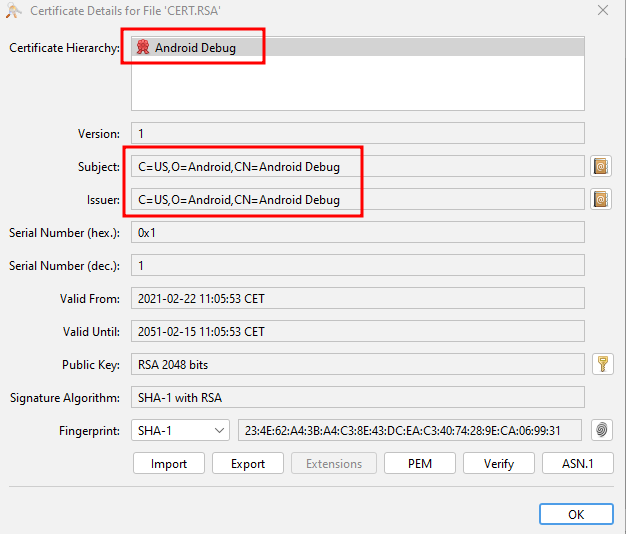
\includegraphics[width=0.7\textwidth,frame]{\CurrentFilePath/DebugCert.png}
\caption{Android debug certificate properties}
\label{figure:DebugCert}
\end{figure}
	

%-<Repeatability>
%-------------------------------------------
%	Countermeasures                        |
%-------------------------------------------



Make sure that release version of the application is signed with the organization certificate of appropriate RSA (2048-bit)
and SHA-2 keysizes.

%-<Countermeasures>
%-------------------------------------------
%	References - pulls bib entries         |
%-------------------------------------------



This finding references the following information sources:

\begin{itemize}
	\item \href{https://doku-center.med.siemens.de/regelwerke/L4U-Intranet/GD/GD-41/GD-41-03-E.pdf}{Siemens Healthineers Guidance for Secure Software Architecture, Design and
	Development: 8.4 Code-Signing}
	\item \bibentry{CWE-296}
\end{itemize}

%-<References>
